\section{Control Structures}

\begin{concept}{Branch Instructions}\\
Branch instructions control program flow:

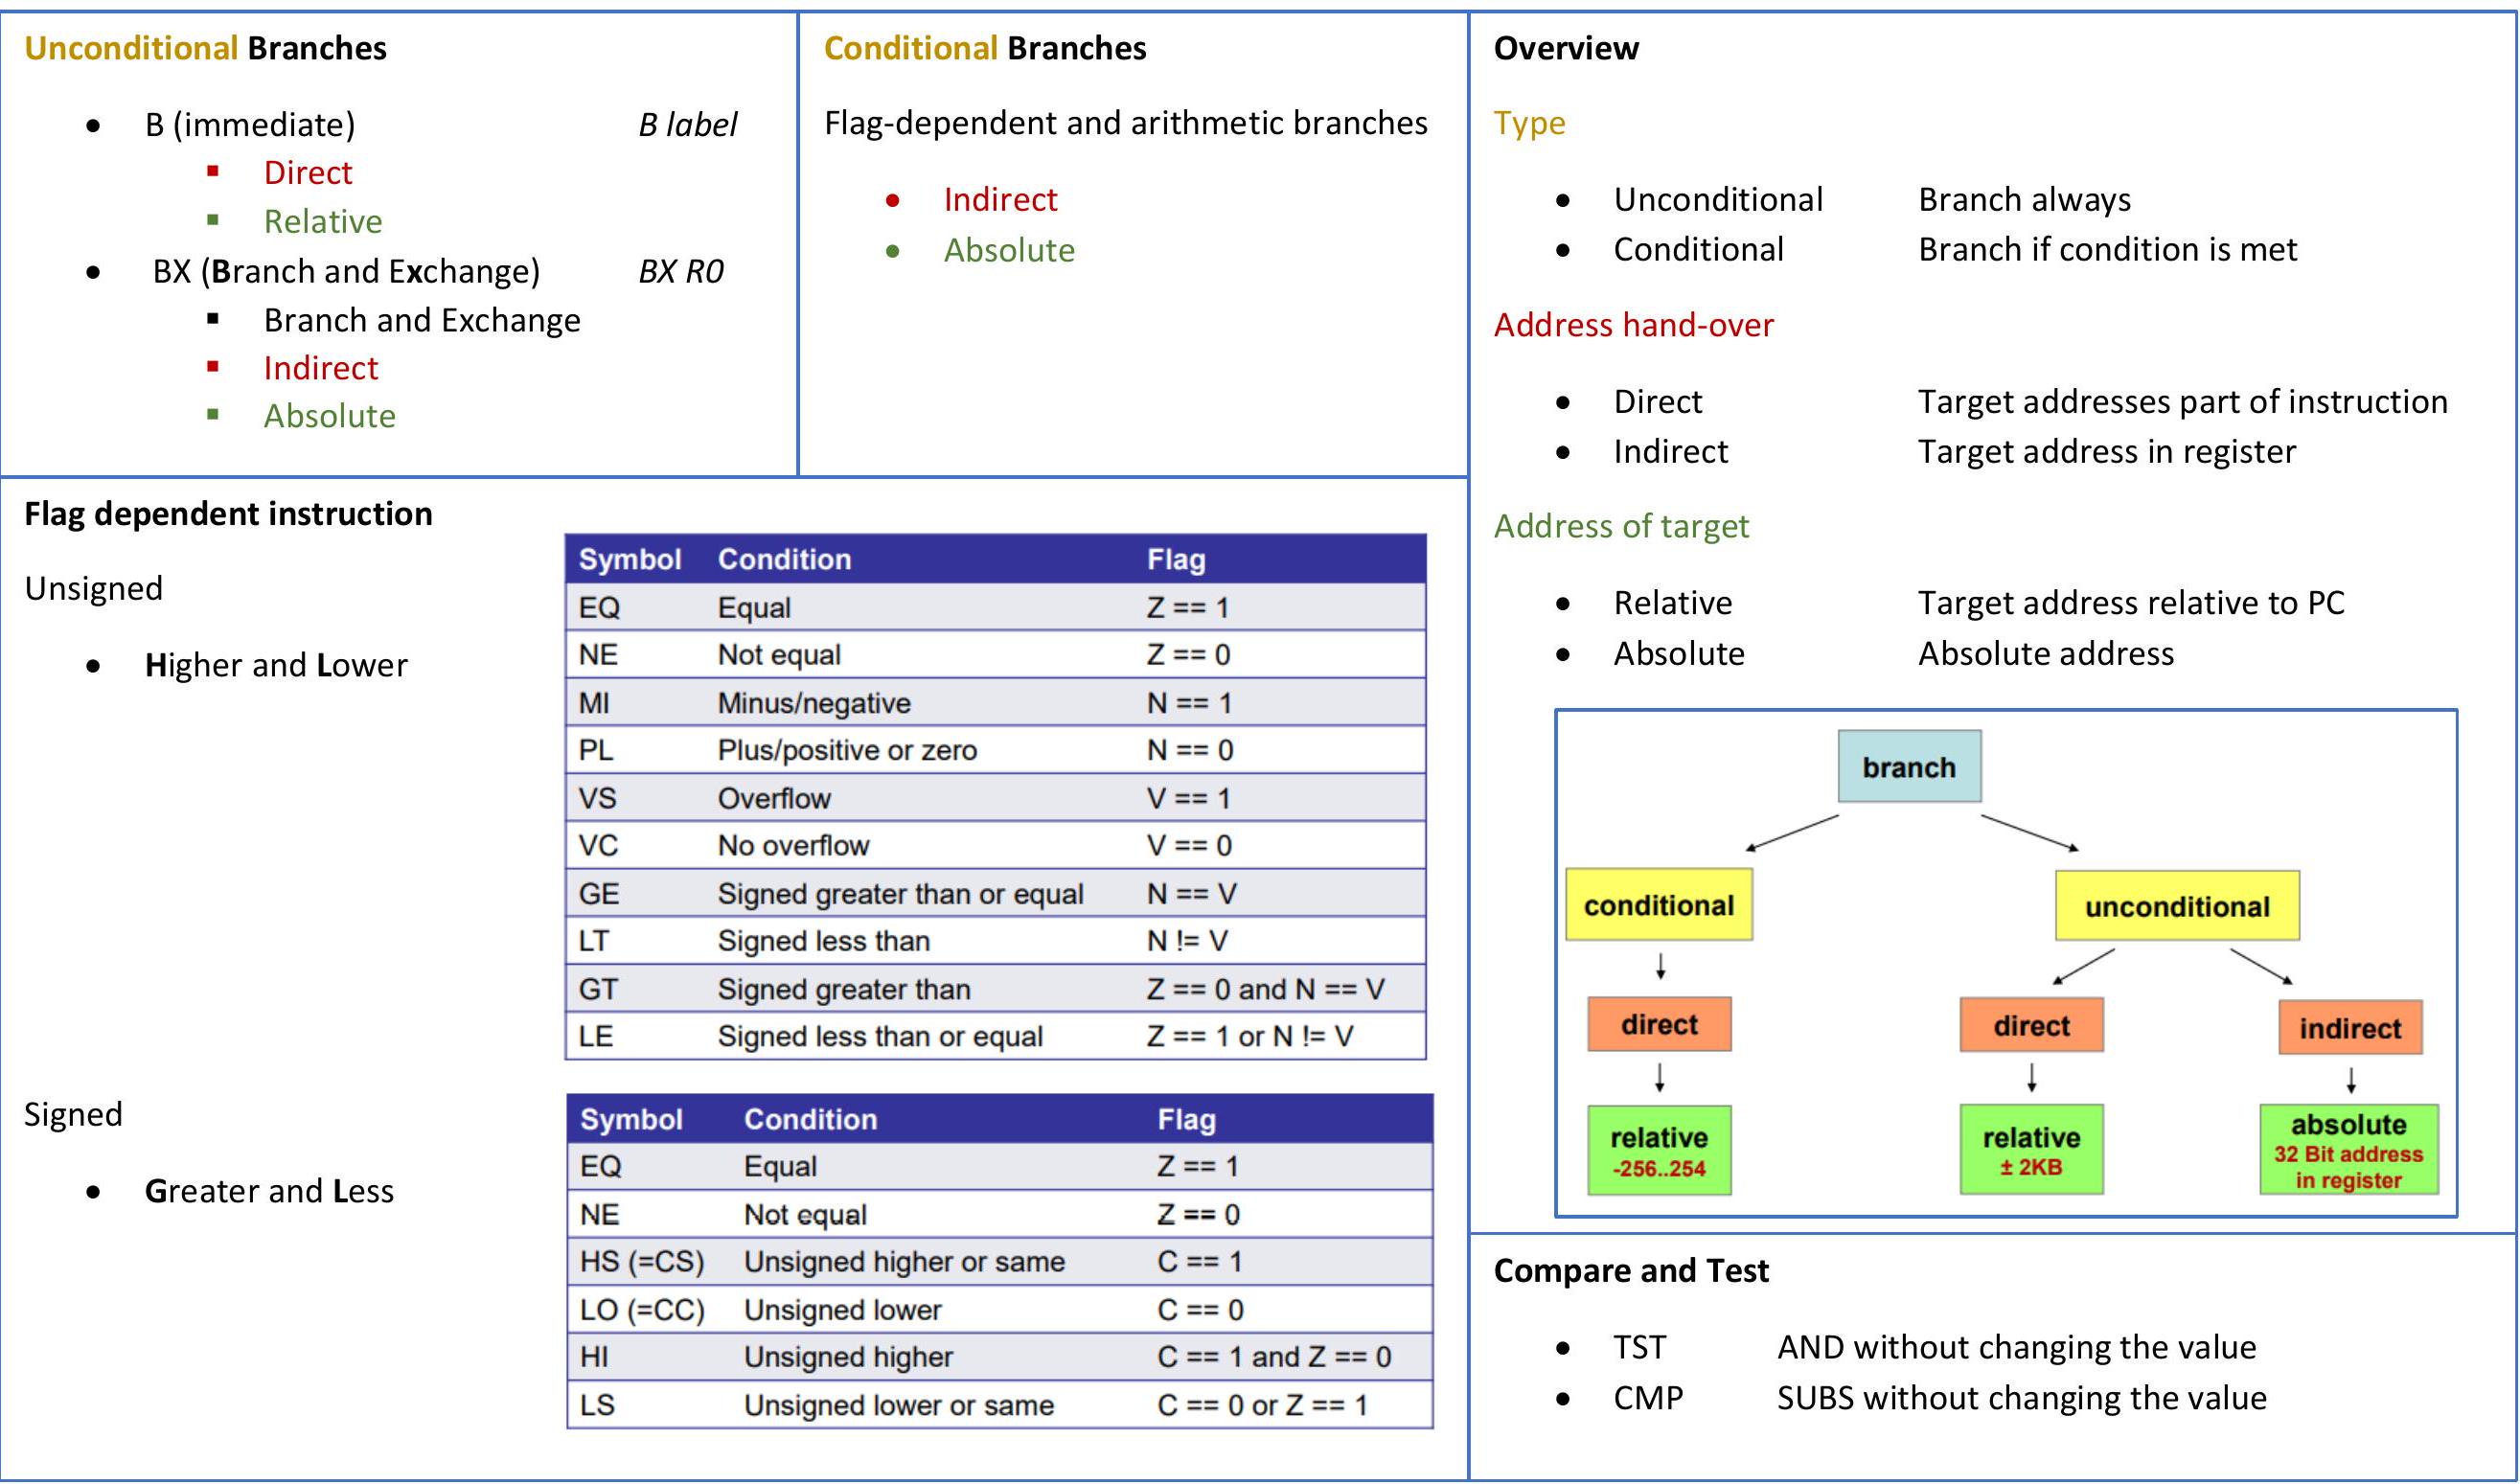
\includegraphics[width=\linewidth]{images/2024_12_29_79e6b22f503fb7b4f718g-05}

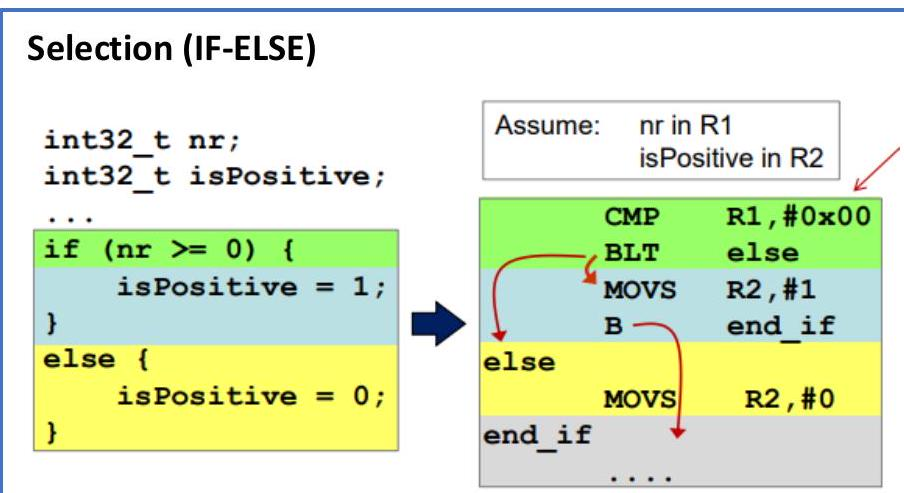
\includegraphics[width=\linewidth]{images/2024_12_29_79e6b22f503fb7b4f718g-07(3)}
\end{concept}

\begin{example2}{Switch Statement Implementation}
C code example:
\begin{lstlisting}[language=C, style=basesmol]
uint32_t result, n;
switch (n) {
    case 0:
        result += 17;
        break;
    case 1:
        result += 13;
        //fall through
    case 3: 
    case 5:
        result += 37;
        break;
    default:
        result = 0;
}
\end{lstlisting}

Assembly implementation with jump table:
\begin{lstlisting}[language=armasm, style=basesmol]
NR_CASES    EQU     6
case_switch CMP     R1, #NR_CASES
            BHS     case_default
            LSLS    R1, #2        ; * 4
            LDR     R7, =jump_table
            LDR     R7, [R7, R1]
            BX      R7

case_0      ADDS    R2, R2, #17
            B       end_sw_case
case_1      ADDS    R2, R2, #13
case_3_5    ADDS    R2, R2, #37
            B       end_sw_case
case_default MOVS   R2, #0
end_sw_case ...

jump_table  DCD     case_0
            DCD     case_1
            DCD     case_default
            DCD     case_3_5
            DCD     case_default
            DCD     case_3_5
\end{lstlisting}
\end{example2}

\begin{concept}{Loop Types}\\
Three main types of loops:

\textbf{Do-While (Post-Test Loop)}:
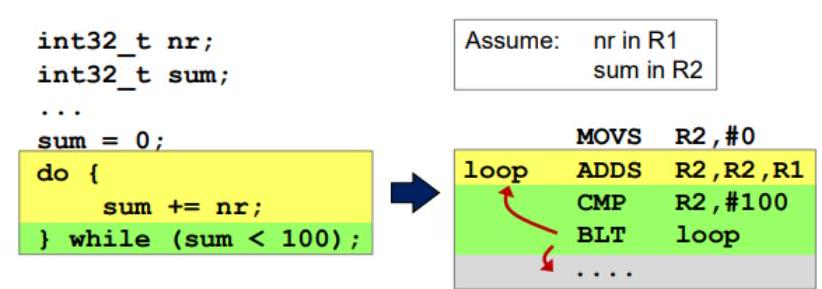
\includegraphics[width=\linewidth]{images/2024_12_29_79e6b22f503fb7b4f718g-07}

\textbf{While (Pre-Test Loop)}:
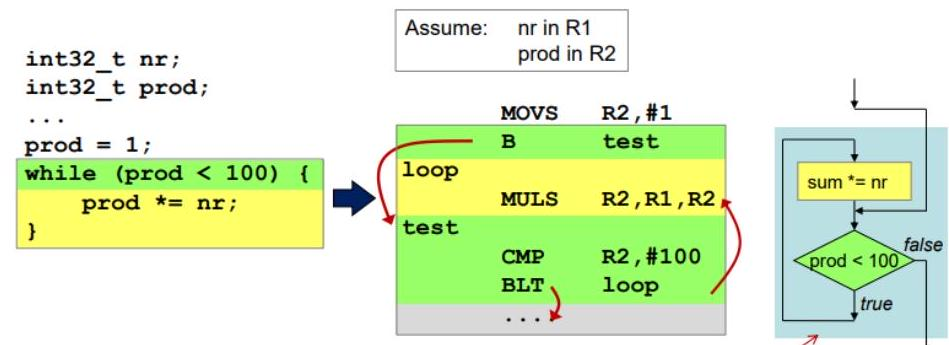
\includegraphics[width=\linewidth]{images/2024_12_29_79e6b22f503fb7b4f718g-07(1)}

\textbf{For Loop (Pre-Test Loop)}:
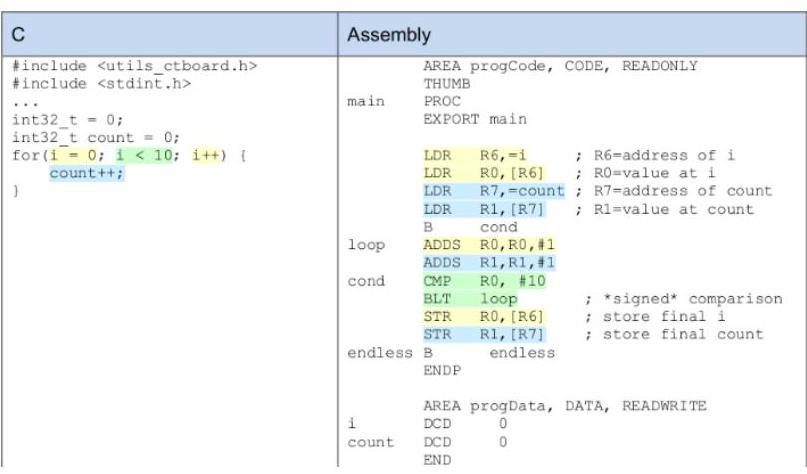
\includegraphics[width=\linewidth]{images/2024_12_29_79e6b22f503fb7b4f718g-07(2)}
\end{concept}

\begin{KR}{Implementing Control Structures}\\
Steps for implementing control structures:
\begin{enumerate}
  \item Choose appropriate control structure:
    \begin{itemize}
      \item If-then-else for simple decisions
      \item Switch for multiple cases with same variable
      \item Loops for repeated operations
    \end{itemize}
  \item For switches:
    \begin{itemize}
      \item Create jump table
      \item Calculate offset based on case value
      \item Handle default case
    \end{itemize}
  \item For loops:
    \begin{itemize}
      \item Initialize counter/condition
      \item Place condition check appropriately
      \item Ensure proper exit condition
      \item Update variables correctly
    \end{itemize}
\end{enumerate}
\end{KR}

\begin{example2}{Basic Control Structures}
Example implementations:
\begin{lstlisting}[language=armasm, style=basesmol]
    ; If-then-else
    CMP     R0, #0      ; Compare value
    BEQ     else_label  ; Branch if equal
    ; then code
    B       endif_label
else_label
    ; else code
endif_label

    ; While loop
    B       while_cond  ; Jump to condition
while_loop
    ; loop body
while_cond
    CMP     R0, #10     ; Check condition
    BLT     while_loop  ; Branch if less than

    ; Do-while loop
do_loop
    ; loop body
    CMP     R0, #10     ; Check condition
    BLT     do_loop     ; Branch if less than
\end{lstlisting}
\end{example2}